When creating test cases to check the validity of the delta function outlined in Section~\ref{sec:overview-delta}. We broke down our test cases to exploit the catagorys of failures on our latice.  Our first constraint of the walk having to begin at (0,0) is tested by the the value of the start state, if the walk could pass this it woudd move out to check for jumps, branches and closure properties. A jump on the latice can happen in one of two ways; horizontal or vertical. A branch has many sub-catagories depending on what is a valid input from the next, the idea is that whatever node the state is currently in can only transfer to one or the other but not both. Closure properties test for self avoding walks, so we created test cases that would demonstrate the delta function knew how to proceed. Out of 60 ran cases below are 4 and how they were logically ran through the delta funtion. 


Figure~\ref{fig:test-branch} demonstrates how the branch condition functions in rejecting an unvalid state. After the start state is processed, for this to be a valid walk it must proceed either from the top or bottom, not both. This is because of the condition that the walk must begin at point (0,0). Once the next input is read into the algorithm this would traverse to the dead state. This is because The branch function detected that this input it received has diverged away from a single path. Once the walk is in the dead state the rest immeditly becomes invalid.
\begin{figure}
\begin{center}
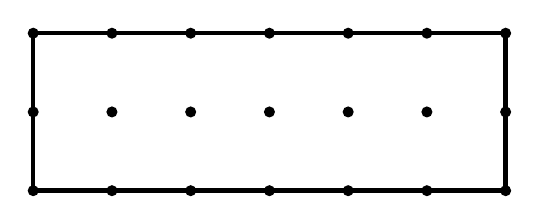
\begin{tikzpicture}
\foreach \x in {0,...,6}
\foreach \y in {0,1,2}
{
\fill (\x,\y) circle (2pt);
}

\draw [ultra thick] (0,0) -- (6,0) -- (6,2) -- (0,2) -- (0,0);

\end{tikzpicture}
\end{center}
\caption{Test case to illustrate branch recognition}
\label{fig:test-branch}
\end{figure}


%%%%%%%%%%%%%%%%%%%%%%%%%%%%%%%%%%%%%%%%%%
Figure~\ref{fig:mult-branch} further shows how the branch condition can detech a unvalid walk. When you receive the input state the only next valid state would be a single node along the bottom. We recvive that making the next valid walk a single node along the top. After the next one however it can easily perceivea branch because it has traversed from the bottom and the middle and not just the top as would have been allowed. This example demonstrates how going from a single node to an illegal tripple node is detected.
\begin{figure}
\begin{center}
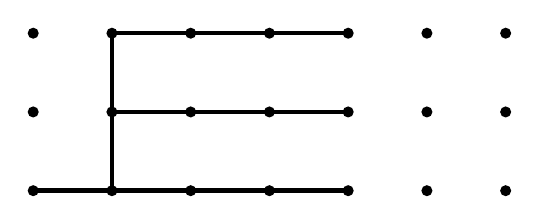
\begin{tikzpicture}
\foreach \x in {0,...,6}
\foreach \y in {0,1,2}
{
\fill (\x,\y) circle (2pt);
}

\draw [ultra thick] (0,0) -- (1,0) -- (2,0) -- (3,0) -- (4,0);
\draw [ultra thick] (1,0) -- (1,1) -- (1,2);
\draw [ultra thick] (1,1) -- (2,1) -- (3,1) -- (4,1);
\draw [ultra thick] (1,2) -- (2,2) -- (3,2) -- (4,2);

\end{tikzpicture}
\end{center}
\caption{Test case to recognize multiple branches}
\label{fig:mult-branch} 
\end{figure}

%%%%%%%%%%%%%%%%%%%%%%%%%%%%%%%%%%%%%%%%%
Figure~\ref{fig:double-ended}is to show how once you have traveled to a double ended state that you must continue to be in any of these double states for the walk to be valid. When the first input is received after the start state is gets a middle bottom path, at this point for example if the algorithm received an input with C=1 (middle and bottom are connected) it would accept. The walk contiues along the double ended state and eventualy receives the proper closure andis then accepted.
\begin{figure}
\begin{center}
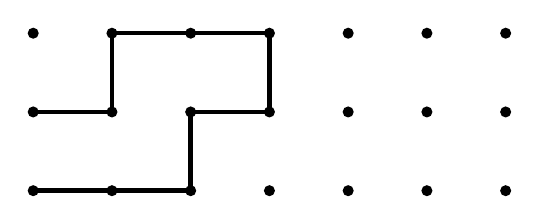
\begin{tikzpicture}
\foreach \x in {0,...,6}
\foreach \y in {0,1,2}
{
\fill (\x,\y) circle (2pt);
}

\draw [ultra thick] (0,0) -- (1,0) -- (2,0) -- (2,1) -- (3,1) -- (3,2) -- (2,2) -- (1,2) -- (1,1) -- (0,1);

\end{tikzpicture}
\end{center}
\caption{Double ended valid walk}
\label{double-ended}
\end{figure}


%%%%%%%%%%%%%%%%%%%%%%%%%%%%%%%%%%%%%%%%
Figure~\ref{fig:tripple-ended} shows a tripple ended state, a valid input from tripple ended state must connect all the nodes to proceed.After the start stateis read, the first input is another tripple ended state and closes two of the paths. This is a valid and the last input we receive so this is a self-avoiding walk. . 
\begin{figure}
\begin{center}
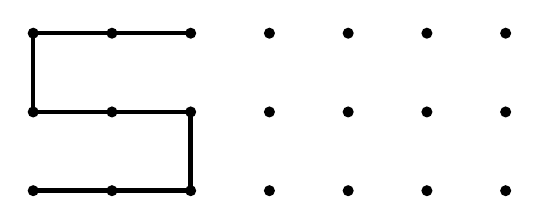
\begin{tikzpicture}
\foreach \x in {0,...,6}
\foreach \y in {0,1,2}
{
\fill (\x,\y) circle (2pt);
}

\draw [ultra thick] (0,0) -- (1,0) -- (2,0) -- (2,1) -- (1,1) -- (0,1) -- (0,2) -- (1,2) -- (2,2);

\end{tikzpicture}
\end{center}
\caption{Tripple-ended}
\label{tripple-ended}
\end{figure}
